\section{Iteration \#1 -- Evaluation Framework, Baselines and the Pyramid Tree}

The first iteration was chosen to be two weeks long, instead of just one. This was to accommodate the extra work that would need to be done initially to lay the foundations that would be used to implement and evaluate the implementations. The objectives for this iteration were:
\begin{itemize}
	\item Design and implement a standard framework for evaluating index in C++
	\item Implement evaluation baselines (Sequential Scan and Octree)
	\item Incorporate the School's implementation of the Pyramid Tree into framework
	\item Analyse performance of two baselines and the Pyramid Tree, evaluating their performance
\end{itemize}

\subsection{Data Generation}

TODO

\subsection{Evaluation Framework}

TODO: discuss design of this, what it does and WHY I decided to do it

TODO: what form an index structure takes -- i.e. its interface

\subsection{Baselines Implementations}

Sequential scan was implemented using the C++ container \texttt{std::vector}, a dynamically resizeable array. Points insertion is $O(1)$ as they are added to the end of the vector and deleting points results in a standard array deletion, making it an $O(n)$ operation. Point queries are performed in $O(n)$ time, as the query iterates through the array sequentially until the given point is found or the end of the array is reached.

The octree variant implemented as a baseline is a bucket PR octree. This means the structure partitions the underlying data space into uniformly sized boxes, without using the points as pivots (unlike point quadtrees or kd-trees). It is a bucket octree because \textit{multiple} points can be stored in a single leaf node. The octree dynamically decomposes and composes spatial regions based on its current contents. When the number of points in a leaf node exceeds a certain number, say $M$, then the region represented by the leaf is sub-divided, creating $2^d$ children. The $M + 1$ points are then scattered across the children. Therefore, regions of space that contain more points are decomposed more and sparse regions of space have less granularity, meaning less nodes and memory overhead. When a point is deleted from a leaf, the contents of the leaf and all of its siblings are checked. If all of these nodes are empty, they are removed and the sub-regions are combined into the original region again. If the now collapsed parent and all of its siblings are empty, then they are collapsed into their parent. This is repeatedly recursively until a parent is reached whose children contain at least one point.

\subsection{Pyramid Tree}

As described in Section \ref{sec:pyramid-tree}, the Pyramid tree reduces multi-dimensional points to one dimension, which can then be used in a one-dimensional index structure. The School of Computing have an existing implementation of the Pyramid tree, written by TODO. While Berchtold et al. in \cite{pyramid-tree} used a B${}^{+}$-tree as the underlying 1D structure, this implementation uses a hash map (specifically \texttt{boost::unordered\_map}). All the points are stored in a single \texttt{std::vector}. Each point is hashed to an integer representation which acts as the key to a bucket stored in the hash map. Each bucket is also a \texttt{std::vector} which contains indices to points in the large point array.

The original Pyramid tree was only created for batch processing (TODO: use official application class here??), which means it was to be used for a single computational task and then discarded. Therefore, \texttt{remove} and \texttt{update} were not implemented. TODO: my version of remove and update

TODO: some optimisations I made??

\subsection{Performance Analysis}

TODO: what I did for the performance analysis, what data I used, operation lists, etc.

TODO: compiler optimisation -- why I decided to not use -O1 

TODO: CPU and heap profiling

TODO: show all the graphs, tables, etc.

\begin{table}
	\centering
	\begin{tabular}{|l|l|l|l|l|l|l|l|l|}
		\hline
		\textbf{Structure} & \textbf{1D} & \textbf{2D} & \textbf{3D} & \textbf{5D} & \textbf{10D} & \textbf{50D} & \textbf{100D} & \textbf{200D} \\
		\hline
		\textbf{Sequential Scan} & 0 & 0 & 0 & 0 & 0 & 0 & 0 & 0 \\
		\textbf{Octree} & 0 & 0 & 0 & 0 & 0 & 0 & 0 & 0 \\
		\textbf{Pyramid Tree} & 0 & 0 & 0 & 0 & 0 & 0 & 0 & 0 \\
		\textbf{Pyramid Tree (No Defragmentation)} & 0 & 0 & 0 & 0 & 0 & 0 & 0 & 0 \\
		\hline
	\end{tabular}
	\caption{Execution Time of Structures for Uniform Randomly Generated Points with \texttt{-O1} Compiler Flag}
	\label{tab:perf1-randuniform-o1}
\end{table}

\begin{table}
	\centering
	\begin{tabular}{|l|l|l|l|l|l|l|l|l|}
		\hline
		\textbf{Structure} & \textbf{1D} & \textbf{2D} & \textbf{3D} & \textbf{5D} & \textbf{10D} & \textbf{50D} & \textbf{100D} & \textbf{200D} \\
		\hline
		\textbf{Sequential Scan} & 0 & 0 & 0 & 0 & 0 & 0 & 0 & 0 \\
		\textbf{Octree} & 0 & 0 & 0 & 0 & 0 & 0 & 0 & 0 \\
		\textbf{Pyramid Tree} & 0 & 0 & 0 & 0 & 0 & 0 & 0 & 0 \\
		\textbf{Pyramid Tree (No Defragmentation)} & 0 & 0 & 0 & 0 & 0 & 0 & 0 & 0 \\
		\hline
	\end{tabular}
	\caption{Execution Time of Structures for Uniform Randomly Generated Points with \texttt{-O3} Compiler Flag}
	\label{tab:perf1-randuniform-o3}
\end{table}
\begin{figure}
	\centering
	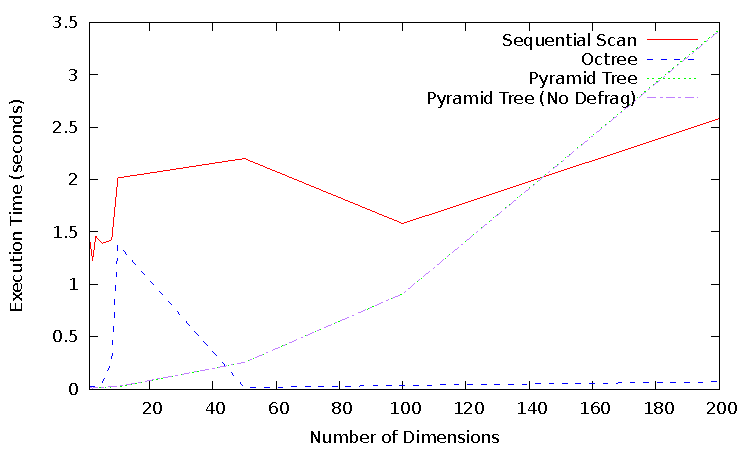
\includegraphics[scale=0.8]{../results/end_of_iteration1/all_insert_randuniform.pdf}
	\caption{\texttt{insert} Performance on Randomly Generated Uniformly Distributed Datasets}
	\label{fig:perf-1-allinsert}
\end{figure}

\begin{figure}
	\centering
	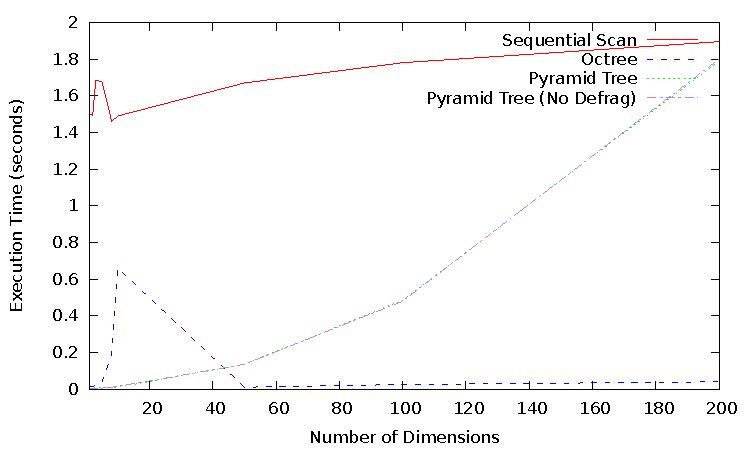
\includegraphics[scale=0.8]{../results/end_of_iteration1/all_pquery_randuniform.pdf}
	\caption{Point Query Performance on Randomly Generated Uniformly Distributed Datasets}
	\label{fig:perf-1-allpquery}
\end{figure}

\begin{figure}
	\centering
	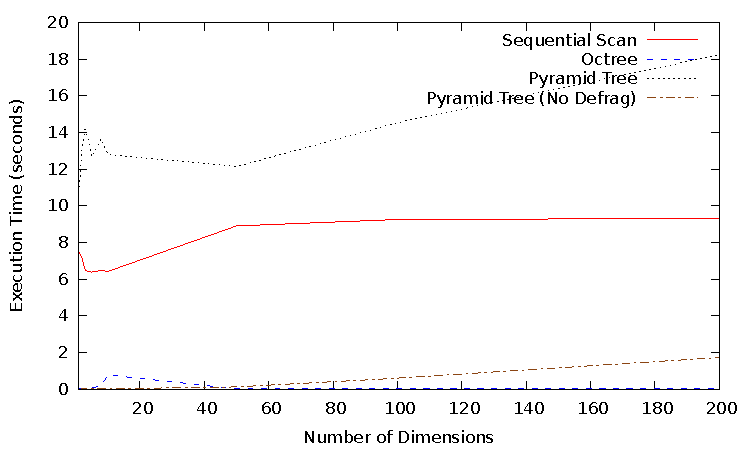
\includegraphics[scale=0.8]{../results/end_of_iteration1/all_delete_randuniform.pdf}
	\caption{\texttt{delete} Performance on Randomly Generated Uniformly Distributed Datasets}
	\label{fig:perf-1-alldelete}
\end{figure}

\subsection{Evaluation}

TODO: evaluate results in previous section

TODO state what was decided to do for next iteration (and why)
